\documentclass[aspectratio=169
%, handout
]{beamer}
%\documentclass[handout]{beamer}
\usetheme{default}

\usepackage[utf8]{inputenc}
\usepackage[ngerman]{babel}
\usepackage{graphicx}
\usepackage{csquotes}
\usepackage{siunitx}
\usepackage{mhchem}
\usepackage{lmodern}
\usepackage{subfig}
 
%\usepackage{scrextend}
%\changefontsizes{18pt}

\usepackage[
backend=biber,
style=authoryear-ibid,
%sorting=ynt
]{biblatex}
\addbibresource{gravitropismus-bibliography.bib}

\author{Alexandra Smirnova}

\title{Präsentation zur Seminararbeit \hyphenquote{ngerman}{Gravitropismus}}
\subtitle{W-Seminar Biologie}

%\title{\hyphenquote{ngerman}{Gravitropismus}}
%\subtitle{Präsentation zum W-Seminar Biologie}

%\logo{}

%\institute{}

\date{19. Dezember 2018}

%\subject{}

\setbeamercovered{transparent}
%\setbeamercovered{invisible}
%\setbeamertemplate{navigation symbols}{}
\setbeamertemplate{section in toc}[sections numbered]
\setbeamertemplate{subsection in toc}[subsections numbered]
\setbeamertemplate{caption}[numbered]


\useoutertheme{infolines}


\makeatletter
\newcommand{\trickbeamer}{%
	\advance\beamer@slideinframe by-1%
}%
\makeatother

\begin{document}
	
	\maketitle
	
	\begin{frame}[<+(1)->]

		\frametitle{Gliederung}
		\pause
		\trickbeamer
		\tableofcontents[pausesubsections,pausesections]
		
	\end{frame}
	
	\section{Grundlagen von Gravitropismus}

	
	\begin{frame}[<+(1)->]
		\frametitle{Gravitropismus}
			\visible<2->{
\begin{figure}[H]
	\centering 
	\includegraphics[width = 0.75\linewidth]{images/gravitrop_reagierende_Pflanze2.pdf}
	%\onslide<2->{\caption{Gravitrop reagierende \emph{Arabidopsis thaliana} \parencite[5]{Masson2002}. Teilabbildung A zeigt den Zustand am Anfang, Teilabbildung B zeigt den Zustand nach vollzogener gravitropischer Reaktion. \label{gravitrop_reagierende_Pflanze}}}
	\caption{Gravitrop reagierende \emph{Arabidopsis thaliana} \parencite[5]{Masson2002}. Teilabbildung A zeigt den Zustand am Anfang, Teilabbildung B zeigt den Zustand nach vollzogener gravitropischer Reaktion. \label{gravitrop_reagierende_Pflanze}}
\end{figure} 
		}
		
	\end{frame}
	
	\subsection{Arten von Gravitropismus}
	
	\begin{frame}[<+(1)->]
		\frametitle{Arten von Gravitropismus}
\begin{enumerate}
\item \textbf{Positiv gravitrop}: zur Schwerkraftquelle hin (nach unten zur Erdmitte)
\item \textbf{Negativ gravitrop}: von der Schwerkraftquelle entgegengesetzt (nach oben)
\item \textbf{Transversalgravitrop}: entweder horizontal oder quer nach unten in einem bestimmten Winkel
\end{enumerate} 
		
\end{frame}
	
\subsection{Prozess der gravitropischen Krümmung}
	
\begin{frame}[<+(1)->]
\frametitle{Prozess der gravitropischen Krümmung in Schritten}
		
\begin{enumerate}
\item \textbf{Reizaufnahme} 
\item \textbf{Signaltransduktion}
\item \textbf{Differenzielles Wachstum}
\end{enumerate}
		
\end{frame}
		
\subsubsection{Reizaufnahme bei Pflanzen durch Statolithen}
		
\begin{frame}[<+(1)->]
\frametitle{Reizaufnahme bei Pflanzen}
\visible<2->{		
	\begin{figure}[H]
		\centering 
		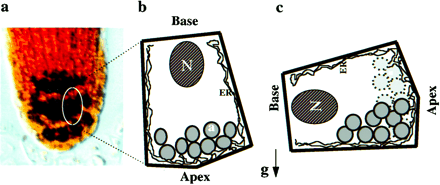
\includegraphics[width = 0.75\linewidth]{images/Statolithen2.png}
		\caption{Statolithen \parencite[345]{Chen1999}. Teilabbildung \textbf{a} zeigt eine Mikroskopaufnahme von Statolithen bei \emph{A. thaliana}. Teilabbildungen \textbf{b} und \textbf{c} zeigen die gravitrope Wirkungsweise von Statolithen, die auf Umlagerung der Amyloplasten bei Veränderung des Schwerkraftvektors beruht. \label{Statolithen}}
\end{figure} }

	\end{frame}

% \begin{frame}[<+(1)->]
% \frametitle{Reizaufnahme bei Pflanzen}
% 
% \begin{enumerate}
% \item Reize durch Statolithen (Amyloplasten, die aus Stärke bestehen)
% \item Statolithen in Statocysten (Statenchyme bei größeren Mengen der Statolithen) in Wurzelspitzen und Innenzellschichten der Sprossachse
% \item Statolithen auf der Membran des endoplasmatischen Retikulums (ER)
% \end{enumerate}
% 
% \end{frame}

% \begin{frame}[<+(1)->]
% \frametitle{Reizaufnahme bei Pflanzen}
% 
%  \begin{figure}[H]
% 	\centering 
% 	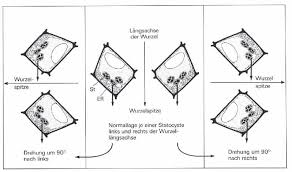
\includegraphics[width = 0.55\linewidth]{images/Graviperzeption.jpeg}
% 	\caption{Querlegen einer Wurzel der Kresse (\emph{Lepidium sativum}). Es erfolgt eine Graviperzeption, in der die Entlastung des Drucks der Membran des ER zu erkennen ist \parencite[533]{Luettge}. \label{Graviperzeption}}
% \end{figure} 
% 
% \end{frame}
			
\subsubsection{Signaltransduktion}
		
% \begin{frame}[<+(1)->]
% 		\frametitle{Signaltransduktion}	
% \begin{enumerate}
% \item Signalübermittlung durch Kontakt zwischen Amyloplasten und ER (gravisensorische Transduktion)
% \item Funktion des Calciums:
% \begin{itemize}
% 	\item \ce{Ca^{2+}}-Efflux durch Druck der Amyloplasten auf die ER-Membran 
% \item Erhöhung der lokalen \ce{Ca^{2+}}-Konzentration im Cytoplasma
% \end{itemize}
% \item Funktion des elektrischen Feldes:
% \begin{itemize}
% 	\item Elektrisches Feld (um die Wurzel herum) durch apoplastischen Strom (Ionenbewegung) 
% \item Bei horizontaler Lage der Pflanze: Änderung des elektrischen Feldes durch die veränderte Richtung des apoplastischen Stroms
% \end{itemize}
% \item Aufnahme des entstandenen Signals (durch die Graviperzeption) in der Streckungszone hinter der Wurzelspitze
% \item Einsetzung der Krümmung beim Ankommen des Signals (ungleiches Wachsen der Flanken)
% \end{enumerate}
% 		
% \end{frame}

\begin{frame}[<+(1)->]
\frametitle{Gravisensorische Signaltransduktion nach Reizaufnahme}

\begin{enumerate}
	\item Kontakt und Druck der \textbf{Amyloplasten} auf die \textbf{ER-Membran}
	\item \textbf{\ce{Ca^{2+}}-Efflux} durch Druck der Amyloplasten auf die ER-Membran 
	\item Erhöhung der lokalen \textbf{\ce{Ca^{2+}}-Konzentration} im Cytoplasma
	\item Änderung des \textbf{elektrischen Feldes}, das die Wurzel umgibt
	\begin{itemize}
		\item Feld entsteht durch Ionenbewegung (\textbf{apoplastischer Strom})
		\item Bei veränderter Pflanzenlage ändert sich die Ionenbewegung und damit das Feld
		\item Aufnahme des entstandenen Signals in der Streckungszone hinter der Wurzelspitze
	\end{itemize}
	
	\item Einsetzung der \textbf{Krümmung} beim Ankommen des Signals (ungleiches Wachsen der Flanken)
\end{enumerate}
\end{frame}
			
\subsubsection{Differenzielles Wachstum}

\begin{frame}[<+(1)->]
\frametitle{Differenzielles Wachstum}
%		\begin{figure}[H]
%			\centering 
%			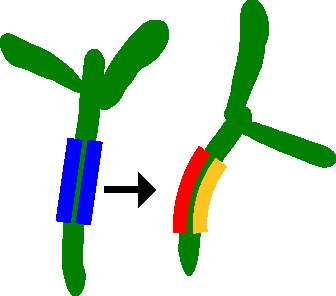
\includegraphics[width = 0.3\linewidth]{images/newdiff.pdf}
%			\caption{Flanken wachsen ungleich (differenziell) nach der Signaltransduktion. Linkes Bild: Flanken gleich groß (blau); rechtes Bild: unterschiedliche Größe der Flanken (rot und orange).}
%		\end{figure} 
\visible<2->{
\begin{figure}
	\begin{minipage}[c]{0.4\textwidth}
		\centering
		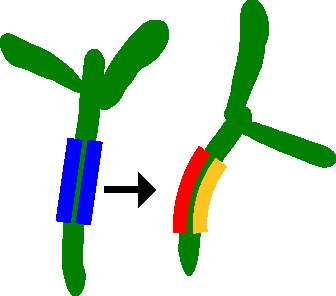
\includegraphics[height=.6\textheight]{images/newdiff.pdf}
	\end{minipage}\hfill
	\begin{minipage}[c]{0.55\textwidth}
		\centering
		\caption{Flanken wachsen ungleich (differenziell) nach der Signaltransduktion. Linkes Bild: Flanken gleich groß (blau); rechtes Bild: unterschiedliche Größe der Flanken (rot und orange).} \label{diffwachs}
	\end{minipage}
\end{figure}
}

\uncover<3->{\begin{itemize}
		\item Wachstumssteuerung durch Auxine und Gibberelline (Pflanzenhormone)
\end{itemize}}



\end{frame}

\begin{frame}[<+(1)->]
\frametitle{Differenzielles Wachstum: Einfluss der Auxine}
\begin{enumerate}
\item \textbf{Synthese} des Auxins im Apikalmeristem 
\item \textbf{Bewegung} der Auxine vom Apikalmeristem bis zur Streckungszone für die \textbf{Stimulierung des Zellwachstums}
\item \textbf{Stimulierung der Protonenpumpe} für die Ansäuerung der Zellwand 
\item \textbf{Aktivierung der Expansine} für die Auflockerung der Zellwand
\item Erhöhte \textbf{Ionenaufnahme} in der Zelle und damit \textbf{Erhöhung des osmotischen Drucks}
\item Mögliche \textbf{Ausdehnung der Zellwand}
\end{enumerate}
\end{frame}
	
\begin{frame}[<+(1)->]
\frametitle{Differenzielles Wachstum: Einfluss der Gibberelline}
\begin{enumerate}
	\item Zusammenwirken der Gibberelline mit Auxin bei der \textbf{Zellstreckung}
	\item \textbf{Aktivierung der Enzyme} für die \textbf{Auflockerung der Zellwand} und für den erleichterten Eintritt der Expansine
\end{enumerate}
\end{frame}

\section{Experimenteller Nachweis von Gravitropismus bei \protect\emph{Lepidium sativum}}
	
\begin{frame}[<+(1)->]
\frametitle{Experimenteller Teil}
\pause
\trickbeamer		
\tableofcontents[currentsection, sections=2, pausesections, pausesubsections, subsectionstyle=show/show/shaded, subsubsectionstyle=show/show/show/shaded]
		
% \begin{enumerate}
% \item Methoden

% 	\item Pflanzen, Materialien und Geräte
%   \item Versuchsmethodik

% \item Durchführung und Ergebnisse
% \item Vorbereitung 
% \item Ankeimen 
% \item Klinostat-Experiment mit Pflanzengruppe 2
% \item Ausrichtungs-Experiment mit Pflanzengruppe 3-5
% \item Diskussion
% \end{enumerate}

\end{frame}	
	
	\subsection{Methoden}
	
	\visible<2->{	\begin{frame}[<+(1)->]
		\frametitle{Methoden}
		\begin{figure}[H]
			\centering 
			\includegraphics[width = 0.5\linewidth]{images/IMG_1044.JPG}
			\caption{Vorbereitung des Experiments und vollständig aufgebautes Klinostat.\label{Klinostat2}}
	\end{figure}}
	
	\end{frame}
	
	\subsubsection{Pflanzen, Material und Geräte}

	\begin{frame}[<+(1)->]
		\frametitle{Pflanzen, Material und Geräte}
\begin{enumerate}
\item Verwendete Pflanze: \textbf{\protect\emph{Lepidium sativum}} (Kresse)
\item Selbstgebautes \textbf{Klinostat}
\item Weitere Materialien: Anzuchtbehälter, Säckchen aus Stoffstück, Plastiktüte, Messzylinder aus Plastik, diverse Gegenstände (z.B. Holzwürfel)
\end{enumerate} 
	\end{frame}

\begin{frame}[<+(1)->]
\frametitle{Aufbau des Klinostats}


% \begin{figure}[H]
% 	\centering 
% 	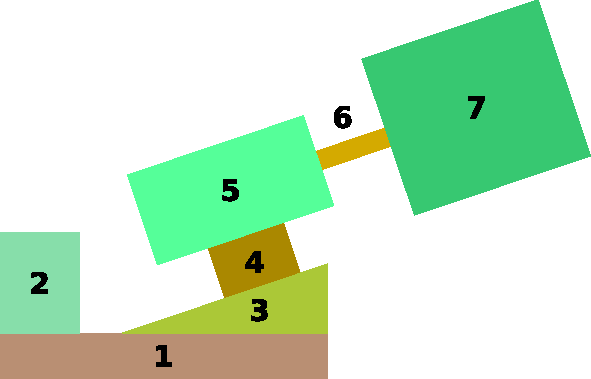
\includegraphics[width = 0.5\linewidth]{images/drawing-1.pdf}
% 	\caption{Schematische Konstruktion des selbst gebauten Klinostats (seitliche Ansicht).}
% 	\end{figure} 

\visible<2->{\begin{figure}
		\begin{minipage}[c]{0.49\textwidth}
			\centering
			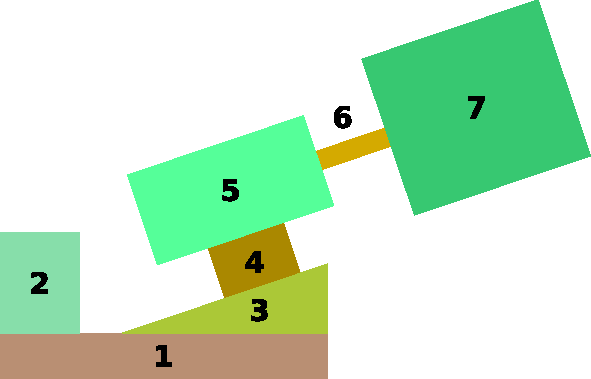
\includegraphics[width=\textwidth]{images/drawing-1.pdf}
		\end{minipage}\hfill
		\begin{minipage}[c]{0.49\textwidth}
			\centering
			\caption{Schematische Konstruktion des selbst gebauten Klinostats (seitliche Ansicht). \\\textbf{1}: \textbf{Befestigungsplatte} (Holz, Dicke: 2cm)\\ \textbf{2}: \textbf{Netzteil} (Modell: MW1000GS, Eingang: 230V~50Hz 28W, Ausgang: 3-6-9-12V, 1000mA 12VA(max))\\ \textbf{3}: \textbf{Holzkeil}, um die Drehachse des Motors um ca. \ang{15} senkrecht zur Ebene anzuheben\\ \textbf{4}: \textbf{Motorbefestigung}\\ \textbf{5}: \textbf{Elektrogetriebemotor} MFA/Como Drills 919D SERIES, single ratio gearbox 3000:1 (Untersetzung 3000:1), 4.5 - 15V DC\\ \textbf{6}: \textbf{Elektromotorwelle}\\\textbf{7}: leere \textbf{Blechdose} mit Öffnung (wird mit einer Muffe an die Elektromotorwelle befestigt)\label{Klinstat1}.} 
		\end{minipage}
\end{figure}}

\end{frame}
	
	\subsubsection{Versuchsmethodik}
	
	\begin{frame}[<+(1)->]
		\frametitle{Versuchsmethodik}
		\framesubtitle{Pflanzengruppen}
\begin{enumerate}
\item Pflanzengruppe 1: \textbf{Kontrollgruppe}
\item Pflanzengruppe 2: Säckchen am \textbf{Klinostat}
\item Pflanzengruppe 3: Anzuchttopf \textbf{kopfüber}
\item Pflanzengruppe 4: Anzuchttopf \textbf{horizontal am Boden}
\item Pflanzengruppe 5: Anzuchttopf \textbf{gewinkelt am Boden} 
\end{enumerate}
		
	\end{frame}
	
\subsection{Durchführung und Ergebnisse}
	
\begin{frame}[<+(1)->]
\frametitle{Durchführung und Ergebnisse}
\framesubtitle{Zeiteinteilung}
		
\begin{enumerate}
\item Versuchstag 1 (28.05.2018): \textbf{Vorbereitung}
\item Versuchstage 2--4 (29.--31.05.2018): \textbf{Ankeimen}
\item Versuchstage 4--5 (31.--01.06.2018): \textbf{Klinostat-Experiment} mit Pflanzengruppe 2
\item Versuchstage 6--7 (02.--03.06.2018): \textbf{Ausrichtungs-Experiment} mit Pflanzengruppen 3--5
\end{enumerate}
\end{frame}
	
\subsubsection{Vorbereitung, Ankeimen}

\begin{frame}[<+(1)->]
\frametitle{Vorbereitung, Ankeimen}
\framesubtitle{Versuchstag 1, 28.05.2018}
		
\begin{enumerate}
\item Bestimmung des \textbf{Versuchsorts}
\item \textbf{Vorbereiten} der vier Anzuchtbehälter + Säckchen 
\item \textbf{Ankeimen} der Kressesamen, bis Sprösslinge stabil wachsen
\end{enumerate}
\end{frame}
	
\subsubsection{Klinostat-Experiment}

\begin{frame}%[<+(1)->]
\frametitle{Klinostat-Experiment}
\framesubtitle{Versuchstage 4--5, 31.05.--01.06.2018}
\begin{columns}
	
	\visible<2->{
		\begin{column}{0.5\textwidth}
			\begin{figure}
	\centering
\includegraphics[width=0.95\linewidth]{images/IMG_1083.JPG}
\caption{Sprossen vor Beginn des Klinostat-Experiments.\label{Foto 1}}		
			\end{figure}
		\end{column}
	}
	\visible<3->{
		\begin{column}{0.5\textwidth}
			\begin{figure}
	\centering		 
\includegraphics[width=0.95\linewidth]{images/IMG_1073.JPG}	
\caption{Sprossen nach Abschalten des Klinostats.\label{Foto 2}}
			\end{figure}
	\end{column}}
\end{columns}
\end{frame}

% 	\begin{frame}[<+(1)->]
% 		\frametitle{Klinostat-Experiment}
% 		
% 	\begin{figure}[H]
% 	\centering
% 	\includegraphics[width=0.5\linewidth]{images/IMG_1083.JPG}
% 	\caption{Sprossen vor Beginn des Klinostat-Experiments.\label{Foto 1}}	
% 	\end{figure}	
% 	
% 	\end{frame}
% 
% \begin{frame}[<+(1)->]
% \frametitle{Klinostat-Experiment}
% 
% \begin{figure}[H]
% 	\centering		 
% 	\includegraphics[width=0.5\linewidth]{images/IMG_1073.JPG}	
% 	\caption{Sprossen nach Abschalten des Klinostats.\label{Foto 2}}
% 	
% \end{figure}
% \end{frame}


\subsubsection{Ausrichtungs-Experiment}
	
\begin{frame}[<+(1)->]
\frametitle{Ausrichtungs-Experiment mit Pflanzengruppen 3--5}
\framesubtitle{Versuchstage 6--7, 02.--03.06.2018}
	
\begin{enumerate}
\item Gruppe 3 \textbf{parallel zum Boden}
\item Gruppe 4 \textbf{kopfüber}
\item Gruppe 5 \textbf{im Winkel von ca. \ang{45} zum Boden}
\end{enumerate}
	
\end{frame}

% \begin{frame}
% \begin{columns}
% 	\column{.5\textwidth}
% 	\visible<1->{
% 		1
% 	}
% 	\column{.5\textwidth}
% 	\visible<2->{
% 				\begin{figure}
% 			\centering
% 			\includegraphics[width=.9\textwidth]{images/A4/IMG_1396.JPG}
% 			\caption{Sprossen am Versuchstag 7.\label{A47}}
% 		\end{figure}
% 	}
% \end{columns}
% \end{frame}

\begin{frame}%[<+(1)->]
\frametitle{Ausrichtungs-Experiment}
\framesubtitle{Pflanzengruppe 3}
\begin{columns}
	
	\visible<2->{
		\begin{column}{0.5\textwidth}
		\begin{figure}
			\centering
			\includegraphics[width=.95\textwidth]{images/A4/IMG_1104.JPG}
			\caption{Sprossen vor Neuausrichtung.\label{A41}}	
		\end{figure}
\end{column}
}
	\visible<3->{
		\begin{column}{0.5\textwidth}
		\begin{figure}
			\centering
			\includegraphics[width=.95\textwidth]{images/A4/IMG_1396.JPG}
			\caption{Sprossen am Versuchstag 7.\label{A47}}
		\end{figure}
\end{column}}
\end{columns}
\end{frame}


% \begin{frame}[<+(1)->]
% \frametitle{Ausrichtungs-Experiment}
% % \begin{figure}[H]
% % \centering
% % \includegraphics[width=0.45\linewidth]{images/A4/IMG_1104.JPG}
% % \caption{Sprossen vor Neuausrichtung.\label{A41}}	
% % \end{figure} 
% 
% \begin{figure}
% 	\centering
% 	\subfloat[First subfigure\label{fig:a}]{\includegraphics[width=3cm]{images/A4/IMG_1104.JPG}}\qquad
% 	\subfloat[Second subfigure\label{fig:b}]{\includegraphics[width=3cm]{images/A4/IMG_1396.JPG}}
% 	\caption{A figure}
% 	\label{fig:1}
% \end{figure}
% 
% \end{frame}
% 
% \begin{frame}[<+(1)->]
% \frametitle{Ausrichtungs-Experiment}
% \begin{figure}[H]
% \centering
% \includegraphics[width=0.45\linewidth]{images/A4/IMG_1396.JPG}
% \caption{Sprossen am Versuchstag 7.\label{A47}}
% \end{figure}
% \end{frame}	

\begin{frame}%[<+(1)->]
\frametitle{Ausrichtungs-Experiment}
\framesubtitle{Pflanzengruppe 4}
\begin{columns}
	
	\visible<2->{
		\begin{column}{0.5\textwidth}
			\begin{figure}
\centering
\includegraphics[width=0.95\linewidth]{images/A3/IMG_1102.JPG}
\caption{Sprossen vor Neuausrichtung.\label{A31}}	
			\end{figure}
		\end{column}
	}
	\visible<3->{
		\begin{column}{0.5\textwidth}
			\begin{figure}
\centering
\includegraphics[width=0.95\linewidth]{images/A3/IMG_1398.JPG}
\caption{Sprossen am Versuchstag 7.\label{A37}}
			\end{figure}
	\end{column}}
\end{columns}
\end{frame}
	
% \begin{frame}[<+(1)->]
% \frametitle{Ausrichtungs-Experiment}
% \begin{figure}[H]
% \centering
% \includegraphics[width=0.5\linewidth]{images/A3/IMG_1102.JPG}
% \caption{Sprossen vor Neuausrichtung.\label{A31}}	
% \end{figure}
% \end{frame}
% 
% \begin{frame}[<+(1)->]
% \frametitle{Ausrichtungs-Experiment}
% \begin{figure}[H]
% \centering
% \includegraphics[width=0.5\linewidth]{images/A3/IMG_1398.JPG}
% \caption{Sprossen am Versuchstag 7.\label{A37}}
% \end{figure}
% \end{frame}

\begin{frame}%[<+(1)->]
\frametitle{Ausrichtungs-Experiment}
\framesubtitle{Pflanzengruppe 5}
\begin{columns}
	
	\visible<2->{
		\begin{column}{0.5\textwidth}
			\begin{figure}
\centering
\includegraphics[width=0.95\linewidth]{images/A5/IMG_1101.JPG}
\caption{Sprossen vor Neuausrichtung.\label{A51}}		
			\end{figure}
		\end{column}
	}
	\visible<3->{
		\begin{column}{0.5\textwidth}
			\begin{figure}
\centering
\includegraphics[width=0.95\linewidth]{images/A5/IMG_1397.JPG}	\caption{Sprossen am Versuchstag 7.\label{A57}}
			\end{figure}
	\end{column}}
\end{columns}
\end{frame}

%\begin{frame}[<+(1)->]
%\frametitle{Ausrichtungs-Experiment}
%\begin{figure}[H]
%\centering
%\includegraphics[width=0.5\linewidth]{images/A5/IMG_1101.JPG}
%\caption{Sprossen vor Neuausrichtung.\label{A51}}		
%\end{figure}
%\end{frame}
%
%\begin{frame}[<+(1)->]
%\frametitle{Ausrichtungs-Experiment}
%\begin{figure}[H]
%\centering
%\includegraphics[width=0.5\linewidth]{images/A5/IMG_1397.JPG}	\caption{Sprossen am Versuchstag 7.\label{A57}}
%\end{figure}
%\end{frame}

\subsection{Diskussion und Fazit}
	
\begin{frame}[<+(1)->]
\frametitle{Diskussion und Fazit}
		
\begin{enumerate}
\item Der gravitrope Effekt ist abhängig von verschiedenen Faktoren:

\begin{itemize}
	\item Sprosslänge 
	\item Stärke des Reizes 
	\item übermäßiger Reiz
	\item Lichteinwirkung 
	\item Reizkonkurrenz
\end{itemize}

\item Unberücksichtigte Faktoren:

\begin{itemize}
	\item Schwankungen in pflanzlichen Hormonen
	\item unterschiedliche Samen
	\item unterschiedliche initiale Wachstumsphasen
	\item Umweltfaktoren wie Druck, Temperatur und Feuchtigkeit
	\item Einflüsse durch das Nährmedium
\end{itemize}

\end{enumerate}
\end{frame}	

\end{document}